\chapter{N$^2$ Charts}
\label{ch:n2_char}

The design of aerospace vehicles is characterised by a multitude of different subsystems with intricate interrelations, its application is suiting for the design of a hybrid UAV. Insight will be provided into input and output parameters between subsystems by means of an N2-chart. This may also allow for a simplification of the system by identifying ineffective or redundant parts. First, in \autoref{sec:subsys} the subsystems are introduced and explained. Then, in \autoref{sec:n2design}, the design N2 chart is explained. Finally in \autoref{sec:n2func} the function N2 chart is illustrated. The difference between both N2 charts is that the functional N2 chart focuses on the functional flow between each of the subsystems during operations, the design N2 chart however explains how the subsystems affect each other during the design of the system. 

\section{Subsystems}
\label{sec:subsys}

In this section, subsystems driving the design of each concept are defined and explained. Seven different subsystems have been created in order to define the entire hybrid Unmanned Aerial Vehicle (UAV) system. \newline

\begin{enumerate}
 \item The propulsion subsystem incorporates engines used for vertical take-off, vertical landing, hovering and horizontal thrust.

\item The structure subsystem consists of all load carrying structures. On top of this, also the main wing, horizontal as well as vertical tailplane and fuselage are included in the structural subsystem. 
\item The flight control subsystem includes all the different parts needed to control the aircraft. This means all high lift devices, the rudder, the ailerons and the flaps as well as eventual thrusters required for control. 

\item The power subsystems main part is the power plant. For an electrical system this will be the battery. However, also energy generation, like solar panels, are part of this subsystem. 

\item The instrumentation subsystem consists of all the sensors to measure important parameters during flight. This amongst others includes temperature, speed, altitude, attitude and pressure sensors. For monitoring missions, also the necessary cameras of the payload are part of this subsystem. 

\item The command and data handling subsystem takes care of all the incoming and outgoing data. It consists of a CPU unit managing data flow from instruments, but also incoming commands from the operators first have to go through this subsystem. 

\item The communication subsystem incorporates devices needed to communicate tasks towards the drone. The operator control system as well as antennas used for communication on the UAV are included in this subsystem. 
\end{enumerate}

\section{Design N2 Chart}
\label{sec:n2design}
In \autoref{fig:N2} one can find the N2 chart which describes how the design of different subsystems change when changing a different subsystem. This system engineering tool is used during the design phase in order to keep a good overview on how the subsystem designs interrelate. The definition of the subsystems from \autoref{fig:N2} can be found in \autoref{sec:subsys}. A brief explanation of the interrelationships is given in the figure and will be elaborated on in this section by referencing to the corresponding numbers. One should note that the N2 chart in this phase of the design is only used for the design of the different subsystems, the actual interrelation during the real operation in missions is included in \autoref{fig:N2}. 

\begin{figure}[htb]
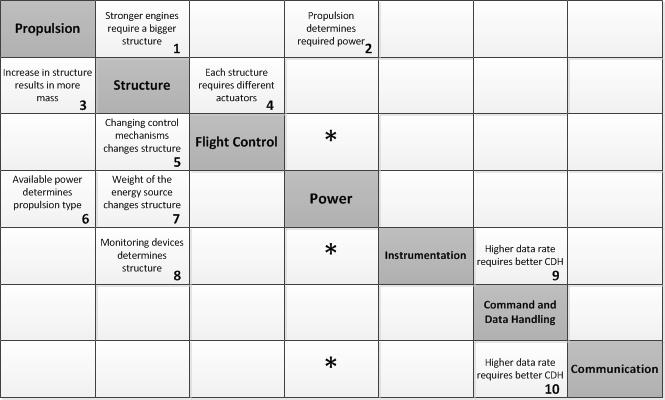
\includegraphics[width=\textwidth]{./Interfaces/Figures/N2Chart.jpg}
\caption{Design N2 Chart}
\label{fig:N2}
\end{figure}

\paragraph{Number 1} In order to integrate the propulsion subsystem in the system, structural support is needed. When for example the weight of the propulsion subsystem increases, more structural support is required. The structures subsystem design will also change when for example the location of the engines changes or the amount of thrust changes.

\paragraph{Number 2} The main power of the UAV is consumed by the propulsion subsystem. This means changing the propulsion engine will require a different energy source as either more or less power will be needed.

\paragraph{Number 3} Changing the structural subsystem of the UAV will also change the mass and external appearance of the system. More mass will lead to more thrust required for VTOL and hovering. A different external appearance will change the aerodynamics flows and hence the drag, requiring a different amount of thrust for horizontal flight. 

\paragraph{Number 4} The instability of the design is mainly determined by the structural subsystem. For example a conventional aircraft without tail-plane will require other means of control for pitching stability. Rotors could be used. After changing the structural design, the stability of the UAV thus has to be analysed again and the necessary actuators, as ailerons, or rotors need to be added. 

\paragraph{Number 5} By changing the control mechanisms of the UAV, different structural components need to be used in order to carry the loads induced by the new control surfaces.


\paragraph{Number 6} When for example due to a constraint the amount of power is limited, a different (more efficient) propulsion system has to be selected in order to be able to provide the required thrust. 


\paragraph{Number 7} A change in the power subsystem, like for example a different type of battery will result in a different take-off mass. This will have an effect on the structure, not only due to the weight, but also due to the volume the power subsystem might take up or the location of the battery. 


\paragraph{Number 8} A change in instrumentation will mean the volume occupied by this subsystem will change. The weight will also change but the volume change will have a greater effect on the structure.


\paragraph{Number 9} The data handling needs to process all the information coming from the instrumentation subsystem, this means that the size of the data handling subsystem needs to be sized for the amount of data coming from the instruments.

\paragraph{Number 10} This relation resembles Number 9, when there is a lot of communication, there is more data to be handled, this will increase the size of the command and data handling subsystem.

\paragraph{*} As it is the case with the propulsion subsystem, the flight control, instrumentation and communication subsystem all determine the amount of power required. However, compared to the power required by the propulsion subsystem, these subsystem use a negligible amount of power. The power subsystem is mainly driven by the required propulsion power requirements. 

\section{Function N2 Chart}
\label{sec:n2func}
Besides the subsystem interface N2 chart, there is also the functional N2 chart. This chart shows for a number of subsystems the functional relationships during operating phase. \autoref{fig:opsN2} shows the function N2 chart of the UAS. Two clear blocks can be distinguished; one related to the ground station and one related to the actual UAV in the operational phase. In can be seen that the connecting element between the two blocks is the 'Command and Data Handling block'.

\begin{figure}[htb]
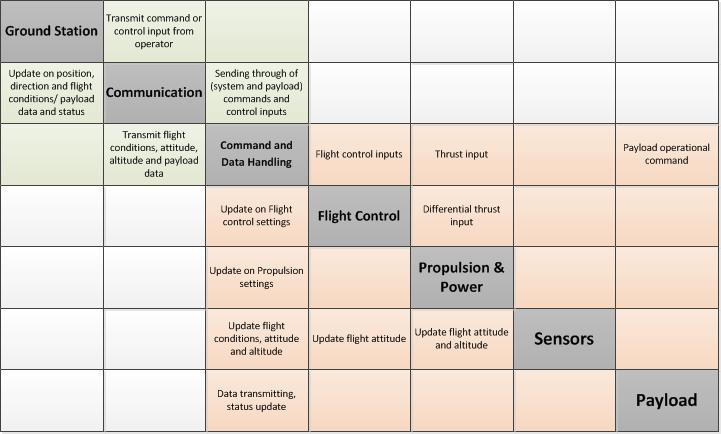
\includegraphics[width=\textwidth]{./Interfaces/Figures/N2ops.jpg}
\caption{Functional N2 Chart}
\label{fig:opsN2}
\end{figure}

The ground station of the UAS, where operator inputs originate from, is connected with the UAV by means of a communication subsystem block. By means of this communication block the the ground station receives status updates of the payload and the UAV (i.e. flight conditions and attitude) and the UAV receives commands or control inputs. All incoming commands are processed by the Command and Data Handling block. All data from the UAV subsystems feed to this block as well. That makes the Command and Data Handling the connecting element between the ground station and the UAV.

Flight Control is the subsystem that proves flight control to the UAV; it enables the UAV to have the required attitude and direction, furthermore it provides stability. This is done either by control surfaces or by means of differential thrust (depending on the flight phase the UAV is in).

The Sensors block is the UAV's connection with its environment; together with the data handling, it enables the UAV to operate autonomously.




